% 圆周运动的加速度

\pentry{圆周运动的速度\upref{CMVD}}

\subsection{匀速圆周运动的加速度(几何法)}

\begin{figure}[ht]
\centering
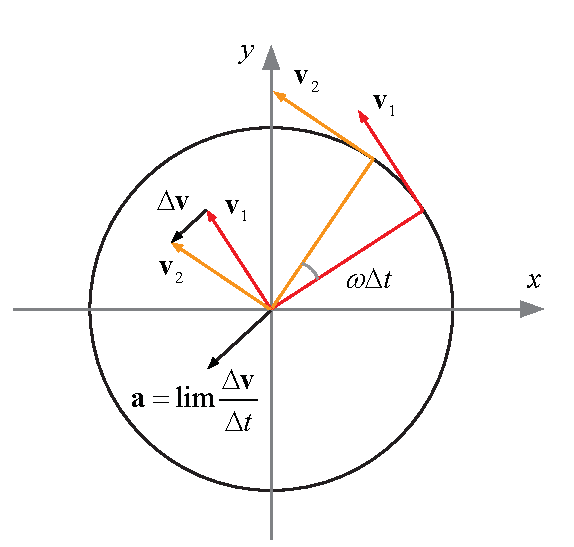
\includegraphics[width=7.5cm]{./figures/CMAD1.pdf}
\caption{把速度矢量移到原点再相减}\label{CMAD_fig1}
\end{figure}

在圆周运动中,位矢 $\bvec r$ 是时间的函数.对时间求导后,我们得到速度矢量关于时间的函数.对速度也进行同样的操作,就不难得到圆周运动的加速度\upref{VnA}.
\begin{equation}
\bvec a = \lim_{\Delta t \to 0} \frac{\Delta \bvec v}{\Delta t}
\end{equation}

现在我们用几何的方法来求该极限.根据矢量减法的定义% 未完成
,计算 $\Delta \bvec v = \bvec v_2 - \bvec v_1$ 要先把 $\bvec v_1$ 和 $\bvec v_2$ 的起点放在一起(例如都放在原点),再从 $\bvec v_1$ 的终点指向 $\bvec v_2$ 的终点得到 $\Delta \bvec v$ (\autoref{CMAD_fig1}). 

我们已知匀速圆周运动的速度大小为 $\abs{\bvec v} = R\omega$, 根据“微小正弦极限\upref{LimArc}”中的结论,把 $\Delta\bvec v$ 的长度用弧长近似,得
\begin{equation}
\abs{\Delta \bvec v} = \abs{\bvec v}\Delta \theta  = (R\omega)\omega \Delta t
\end{equation}
所以质点的加速度大小为
\begin{equation}
a =\lim_{\Delta t \to 0} \frac{\abs{\Delta \bvec v}}{\Delta t} =  \lim_{\Delta t \to 0} \frac{\omega ^2 R \Delta t}{\Delta t} = \omega ^2 R
\end{equation}
由图可得加速度的方向是速度方向逆时针偏转 $\pi/2$. 又由于速度方向是位移方向逆时针偏转 $\pi/2$,所以匀速圆周运动的加速度的方向与位矢的方向相反.

结合模长和方向,令 $\bvec r$ 为位矢(取圆心为坐标原点),就得到加速度的矢量形式
\begin{equation}\label{CMAD_eq4}
\bvec a =  - \omega ^2 \bvec r
\end{equation}

\subsection{圆周运动的加速度(求导法)}
现在我们来推导一般圆周运动的加速度(不要求匀速),  将\autoref{CMVD_eq2}\upref{CMVD} 继续对时间求导得加速度
\begin{equation}
\bvec a = \dot {\bvec v} =  - R \dot\theta^2(\cos \theta\, \uvec x + \sin \theta\, \uvec y) + \ddot\theta R [\cos(\theta + \pi/2) \uvec x + \sin(\theta + \pi/2)\uvec y]
\end{equation}
当角速度 $\omega = \dot\theta$ 为常量时(匀速圆周运动), 上式第二项为零, 第一项与\autoref{CMAD_eq4} 相同, 当角速度随时间变化时, 由于 $\ddot\theta R = \dot\omega R = \dot v$, 上式可以记为
\begin{equation}\label{CMAD_eq6}
\bvec a = - \omega ^2 \bvec r + \dot v \uvec v
\end{equation}
其中 $\uvec v$ 是速度方向的单位矢量. 所以变速圆周运动除了向心加速度外, 还有一个沿速度方向的加速度.

\subsection{三维空间的情况}
\pentry{连续叉乘的化简\upref{TriCro}}
若要把\autoref{CMAD_eq4} 拓展到三维空间中围绕过圆心的轴转动的任意匀速圆周运动, 可以对\autoref{CMVD_eq5}\upref{CMVD} 求时间导数(令 $\bvec\omega$ 为常矢量)得
\begin{equation}\label{CMAD_eq7}
\bvec a = \dot{\bvec v} = \bvec\omega \cross \bvec v
\end{equation}
将\autoref{CMVD_eq5}\upref{CMVD} 代入上式, 得
\begin{equation}\label{CMAD_eq9}
\bvec a =  \bvec\omega \cross (\bvec\omega \cross \bvec r)
\end{equation}
要验证该式与\autoref{CMAD_eq4} 吻合, 把连续叉乘化为内积得
\begin{equation}
\bvec a = \omega^2 r \cos\theta\, \uvec \omega - \omega^2 \bvec r = -\omega^2 (\bvec r - r\cos\theta\, \uvec\omega) = -\omega^2 \bvec r_\bot
\end{equation}
其中 $\theta$ 是 $\uvec\omega$ 和 $\uvec r$ 之间的夹角, $\bvec r_\bot$ 是从圆周运动的圆心指向点 $P$ 的矢量, 相当于\autoref{CMAD_eq4} 中的 $\bvec r$. 证毕.

我们再来考虑变速圆周运动的情况, 当 $\bvec\omega$ 的模长随时间变化时, \autoref{CMAD_eq7} 变为
\begin{equation}
\bvec a = \bvec\omega \cross \bvec v + \dot{\bvec\omega} \cross \bvec r 
\end{equation}
定义\bb{角加速度} $\bvec\alpha = \dot{\bvec\omega}$, 并将\autoref{CMVD_eq5}\upref{CMVD} 代入, 得
\begin{equation}
\bvec a =  \bvec\omega \cross (\bvec\omega \cross \bvec r) + \bvec\alpha\cross\bvec r
\end{equation}
由定义易证右边第二项等于\autoref{CMAD_eq6} 中的 $\dot v\uvec v$.




